\appendix
\section*{Appendix}
\addcontentsline{toc}{section}{Appendix}



\section{Harness Interface Signatures}
\label{sec:harness-signatures}

\begin{table}[H]
\centering
\caption{Harness interface signatures.}
\label{tab:harness-interfaces}
\small
\setlength{\tabcolsep}{4pt}
\begin{tabularx}{\textwidth}{@{}>{\ttfamily\raggedright\arraybackslash}p{0.16\textwidth}>{\raggedright\arraybackslash}p{0.38\textwidth}X@{}}
\toprule
\textbf{Interface} & \textbf{Signature} & \textbf{Responsibility} \\
\midrule
Execution & \texttt{execute(task, ctx) $\to$ (result, cost)} & Dispatch task to backend, return output \\
\addlinespace
Task & \texttt{enqueue(task); dequeue() $\to$ task} & Per-employee queue, mutual exclusion \\
\addlinespace
Event & \texttt{publish(event); subscribe(filter)} & Organisational event bus \\
\addlinespace
Storage & \texttt{read(key) $\to$ data; write(key, data)} & Persistent memory (short/medium-term) \\
\addlinespace
Context & \texttt{assemble(role, guidance, memory) $\to$ ctx} & Execution context construction \\
\addlinespace
Lifecycle & \texttt{pre\_hook(task, ctx); post\_hook(task, result)} & Validation, guardrails, self-improvement \\
\bottomrule
\end{tabularx}
\end{table}

\section{Harness--OS Kernel Correspondence}
\label{sec:os-mapping}

The six Harness interfaces correspond to the canonical subsystems of an OS kernel as identified in standard references~\cite{tanenbaum2014modern, silberschatz2018os}.  Table~\ref{tab:os-correspondence} maps each kernel subsystem to the Harness interface(s) that fulfil the analogous role for agent workforces.

\begin{table}[H]
\centering
\caption{Mapping from classical OS kernel subsystems to OMC Harness interfaces.}
\label{tab:os-correspondence}
\small
\setlength{\tabcolsep}{4pt}
\begin{tabularx}{\textwidth}{@{}>{\raggedright\arraybackslash}p{0.17\textwidth}>{\raggedright\arraybackslash}p{0.20\textwidth}>{\ttfamily\raggedright\arraybackslash}p{0.14\textwidth}X@{}}
\toprule
\textbf{OS Subsystem} & \textbf{Kernel Responsibility} & \textbf{Harness Interface} & \textbf{OMC Realisation} \\
\midrule
Process Mgmt. & Create, schedule, and terminate processes & Execution, Task & Dispatch tasks to Vessels; enforce mutual exclusion ($|\text{running}(e)| \leq 1$); manage per-employee task queues with enqueue/dequeue semantics \\
\addlinespace
Memory Mgmt. & Allocate address spaces; isolate process memory & Context & Assemble the execution context (role identity, working principles, accumulated memory) each agent sees at runtime \\
\addlinespace
File System & Persistent storage with uniform read/write API & Storage & Uniform \texttt{read}/\texttt{write} over heterogeneous backends (YAML profiles, progress logs, memory stores) \\
\addlinespace
I/O \& Device Mgmt. & Abstract heterogeneous hardware behind driver interfaces & Vessel contract & Each Vessel type implements the six Harness interfaces so the platform never touches backend-specific APIs \\
\addlinespace
IPC & Message passing, signals, shared memory & Event & Publish--subscribe event bus for organisational events across all agents \\
\addlinespace
Security \& Audit & Policy enforcement, access control, accounting & Lifecycle & Pre-task hooks enforce guardrails and input validation; post-task hooks perform self-reflection and audit logging \\
\bottomrule
\end{tabularx}
\end{table}


\section{Executor Backends and Task Dispatch}
\label{sec:execution}
% ─────────────────────────────────────────────────────────────────────

\paragraph{On-Demand Dispatch.}
Agents do not poll for work. Tasks are dispatched on demand: execution begins immediately through the harness sequence when a task is assigned, and the agent consumes no resources when idle. The system scales naturally---adding agents does not increase idle overhead---and recovers from interruptions because all state is persisted rather than held in running processes.

\paragraph{Three Reference Backends.}
The \texttt{ExecutionHarness} decouples task dispatch from the agent runtime. Three reference implementations are provided: (1)~a LangChain-based reactive agent for tool-using tasks, (2)~a Claude Code session for long-horizon reasoning, and (3)~a script-based executor for lightweight or custom runtimes. Because the harness carries all state, each executor is kept stateless and minimal. Additional backends can be registered without changes to existing agents or infrastructure.

\paragraph{Failure Recovery.}
When an agent fails a task, the failure is captured, error context is injected into the retry prompt, and execution resumes with updated information. After a configurable number of attempts, the task is escalated to the supervising agent for review and reassignment. This recovery loop operates entirely through harness interfaces, so the behavior is consistent across executor backends.

% ─────────────────────────────────────────────────────────────────────
\subsection{Tool and Skill System}
\label{sec:tools}
% ─────────────────────────────────────────────────────────────────────

\paragraph{Role-Based Tool Access.}
An agent's action space is determined by which tools it is authorized to use. The system enforces this through a unified tool registry that gates access by role, explicit permission grants, and asset ownership. Permissions are resolved at prompt assembly time: each agent's context includes only authorized tools, so capability boundaries are enforced before the agent begins reasoning.

\begin{table}[H]
\centering
\caption{Tool permission categories}
\label{tab:tools}
\small
\setlength{\tabcolsep}{4pt}
\begin{tabularx}{\textwidth}{@{}>{\raggedright\arraybackslash}p{0.16\textwidth}>{\raggedright\arraybackslash}p{0.31\textwidth}X@{}}
\toprule
\textbf{Category} & \textbf{Access Rule} & \textbf{Examples} \\
\midrule
Base & All employees & \texttt{dispatch\_child}, \texttt{accept\_child}, \texttt{read\_file} \\
Gated & Requires \texttt{tool\_permissions} in profile & Email integration, external API access \\
Role & Employee role $\in$ \texttt{allowed\_roles} & \texttt{code\_review} (Reviewer), design tools (Designer) \\
Asset & \texttt{allowed\_users} includes employee ID & Company-specific tools, Talent-provided tools \\
\bottomrule
\end{tabularx}
\end{table}

\paragraph{Cross-Backend Tool Exposure.}
Tools are exposed through a standard interface regardless of executor backend. For Claude Code sessions, tools are surfaced via the Model Context Protocol (MCP), allowing the same organizational capabilities as LangChain-based agents. From the harness perspective, MCP bridging is an implementation detail of one executor---the tool contract is uniform across backends.

\paragraph{Tools as Inter-Agent Coordination.}
Core inter-agent tools cover the full range of organizational interaction: delegating work to a subordinate, accepting or rejecting a subtask, convening a multi-agent discussion, and escalating a decision to the CEO. Each interaction is expressed as a tool call that flows through the harness layer and produces effects visible to all agents.

\section{Talent Market: A Three-Type Agent Supply Chain}
\label{sec:talent-supply}
% ─────────────────────────────────────────────────────────────────────

The Talent Market is the supply-side complement to the Vessel abstraction: while the Vessel defines \emph{how} an agent executes, the Talent Market determines \emph{what} cognitive capability is available for hire. It provides three types of agent sourcing, each representing a different method of constructing a Talent package. The three types are not ranked by quality or priority---they are parallel supply channels, and all produce standard Talent packages that enter the OMC runtime through the same pathway: loaded into a Vessel and governed by the Harness interfaces. Once hired, every agent begins at the same employee level regardless of its sourcing type.

\paragraph{Type 1: Curated Repository Agents.}
Type~1 agents are manually packaged from established open-source agent repositories. Each source project is selected based on community adoption metrics and benchmark performance; its core reasoning strategies, tool interfaces, and domain knowledge are distilled into the OMC Talent package format, stripping framework-specific runtime dependencies. The resulting Talents are validated against reference tasks to ensure behavioral fidelity. This sourcing method is best suited for domains where mature, battle-tested agent implementations already exist in the open-source ecosystem.

\paragraph{Type 2: Prompt-Sourced Agents with Skill Assembly.}
Type~2 agents start from high-quality \emph{system prompts} sourced from community-curated prompt repositories---notably the Agency-Agents collection~\cite{agencyagents}, which provides over 140 specialist personas spanning engineering, design, marketing, product, sales, project management, testing, and other divisions. Each persona defines a detailed identity, working principles, deliverable specifications, and success metrics, but carries no executable tool bindings or runtime skills. To transform a persona into a deployable Talent, OMC applies an automated \textbf{skill assembly} step: the system queries the SkillsMP marketplace~\cite{skillsmp} using the persona’s domain descriptors and capability requirements as a structured search query, retrieves compatible skills (tool bindings, behavioral principles, workflow fragments), and composes them with the source persona into a complete Talent package. This sourcing method is best suited when a well-defined role description exists but no complete agent implementation is available.

\paragraph{Type 3: Dynamic Agent Assembly from Cloud Skills.}
Type~3 agents are assembled entirely from modular skills retrieved from SkillsMP~\cite{skillsmp}, an open community-driven skill marketplace that aggregates agent skills from public GitHub repositories using the standardized \texttt{SKILL.md} format. Unlike Type~1 (which packages an existing implementation) or Type~2 (which starts from a curated persona), Type~3 constructs \emph{both} the persona and the skill set on demand. The HR agent provides a structured job description based on the task specification; the Talent Market then performs semantic search over skill metadata, filters for mutual compatibility and harness compliance, ranks by relevance and community score, and synthesizes a coherent agent identity from the retrieved components. This sourcing method is best suited for niche or emerging domains where neither complete agent implementations nor established persona templates yet exist, and also serves as a \emph{cold-start} mechanism for the Talent Market as a whole.

\paragraph{Human-in-the-Loop Talent Selection.}
Talent hiring is not fully automated: the system presents a ranked \emph{top-$k$} recommendation list to the CEO, who makes the final selection. To ensure the CEO sees a diverse range of sourcing methods, the recommendation engine composes the shortlist with an approximately 80/20 distribution---roughly 80\% of candidates from Type~1 and Type~2, and 20\% from Type~3. This ratio reflects the current relative maturity of each supply channel rather than an intrinsic quality ordering: Type~1 and Type~2 draw from repositories with established community validation, while Type~3’s dynamically assembled agents offer broader coverage but have not undergone prior community review. The CEO can inspect each candidate’s provenance---source repository for Type~1, source persona and attached skills for Type~2, constituent skills for Type~3---and approve or reject before the hiring pipeline provisions a Vessel.

\paragraph{Cross-Type Feedback.}
The three sourcing channels are not isolated: skills refined through deployed agents’ self-improving loops can be published back to the skill marketplace, enriching the community pool regardless of which type originally produced the agent. Similarly, a Type~3 agent whose synthesized persona proves effective across multiple projects can have that persona persisted and contributed to prompt repositories, expanding the available pool for future Type~2 sourcing.


\section{GitHub AI Agent Weekly Trend Report}
\label{appendix:github-report}

The following report was autonomously produced by the Writer agent (Claude Sonnet~4)
in the content-generation case study (Section~\ref{sec:case-content}), based on
research data collected by the Researcher agent (GPT-4o) and subsequently emailed
to the CEO without human editing.

\begin{mdframed}[
  linewidth=0.8pt,
  linecolor=black!40,
  backgroundcolor=black!2,
  innertopmargin=16pt,
  innerbottommargin=16pt,
  innerleftmargin=18pt,
  innerrightmargin=18pt,
  roundcorner=4pt
]
\sloppy
{\centering
  {\large\bfseries GitHub AI Agent Trending Repositories Report}\\[4pt]
  {\normalsize\bfseries Past Week Analysis (March 18--25, 2026)}\\[2pt]
  \textit{\small Researcher: GPT-4o\quad|\quad Writer: Claude Sonnet~4\quad|\quad Generated: March 25, 2026}
\par}

\vspace{8pt}
\hrule height 0.4pt
\vspace{10pt}

\noindent\textbf{Executive Summary}

\noindent
This comprehensive report analyzes the most significant AI Agent repositories that gained traction on GitHub during the past week (March 18--25, 2026). Our research identified 15 notable repositories spanning from enterprise-grade solutions to specialized domain applications, representing a total of over 4,000 stars across all projects.

\vspace{8pt}
\noindent\textbf{Key Market Trends}

\noindent\textit{Multi-Platform Integration Dominance.}\quad
The most significant trend is the surge in cross-platform agent integrations, particularly targeting Chinese market platforms: \textbf{weixin-agent-sdk} (887 stars) --- WeChat Clawbot integration; \textbf{astronclaw-tutorial} (268 stars) --- AstronClaw \& Loomy AI assistant tutorials.

\vspace{4pt}
\noindent\textit{Agent-to-Agent Communication Revolution.}\quad
A new paradigm is emerging with autonomous agent collaboration: \textbf{ClawLink} (246 stars) --- AI Agent Social Network enabling direct agent-to-agent communication; \textbf{HyperAgents} (784 stars) --- Self-referential self-improving agents.

\vspace{4pt}
\noindent\textit{Specialized Domain Applications.}\quad
Agents are becoming increasingly specialized: \textbf{app-store-preflight-skills} (936 stars) --- App Store compliance scanning; \textbf{ctf-agent} (194 stars) --- Autonomous CTF solver (1st place BSidesSF 2026); \textbf{buzz-bd-agent} (4 stars) --- Business development automation.

\vspace{8pt}
\noindent\textbf{Top Performing Repositories}

\vspace{4pt}
\noindent\textit{Most Popular (500+ Stars)}

\vspace{2pt}
\noindent\textbf{1.~app-store-preflight-skills} $\bigstar$~936\quad
\url{https://github.com/truongduy2611/app-store-preflight-skills}\\
AI agent skill for scanning iOS/macOS projects for App Store rejection patterns. Addresses a critical pain point for mobile developers.

\vspace{4pt}
\noindent\textbf{2.~weixin-agent-sdk} $\bigstar$~887\quad
\url{https://github.com/wong2/weixin-agent-sdk}\\
Clawbot WeChat integration for any Agent. Opens Chinese market access for global AI agents.

\vspace{4pt}
\noindent\textbf{3.~HyperAgents} $\bigstar$~784\quad
\url{https://github.com/facebookresearch/HyperAgents}\\
Self-referential self-improving agents for any computable task. Represents a breakthrough in autonomous self-improvement.

\vspace{6pt}
\noindent\textit{High Growth Projects (200--500 Stars)}

\vspace{2pt}
\noindent\textbf{4.~cc-skills-golang} $\bigstar$~281\quad \url{https://github.com/samber/cc-skills-golang}\quad Golang agentic skills collection.

\noindent\textbf{5.~astronclaw-tutorial} $\bigstar$~268\quad \url{https://github.com/iflytek/astronclaw-tutorial}\quad Complete tutorial for AstronClaw (cloud) \& Loomy (desktop) AI.

\noindent\textbf{6.~ClawLink} $\bigstar$~246\quad \url{https://github.com/CN-Syndra/ClawLink}\quad AI Agent Social Network for autonomous agent communication.

\noindent\textbf{7.~agent-kernel} $\bigstar$~226\quad \url{https://github.com/oguzbilgic/agent-kernel}\quad Minimal kernel for stateful AI coding agents.

\vspace{8pt}
\noindent\textbf{Emerging Innovation Areas}

\noindent\textit{Infrastructure \& Tooling}:\quad \textbf{usecomputer} (136 stars) --- Fast computer automation CLI; \textbf{agent-kanban} (22 stars) --- Mission control for AI workforce.

\noindent\textit{Security \& Compliance}:\quad \textbf{ctf-agent} (194 stars) --- Autonomous CTF solver; \textbf{copilot-cli-knowledge-agents} (2 stars) --- 13 specialized agents with security council.

\noindent\textit{Development Workflow}:\quad \textbf{spec\_driven\_develop} (189 stars) --- Spec-driven development; \textbf{flyai-skill} (171 stars) --- Alibaba's fly AI agent skill collection.

\vspace{8pt}
\hrule height 0.4pt
\vspace{8pt}

\noindent\textbf{Conclusion}\quad
The past week demonstrates accelerating innovation across platform integration (especially Chinese markets), agent autonomy (self-improvement and collaboration), enterprise applications, and infrastructure maturation. The total engagement of 4,000+ stars across 15 repositories indicates strong developer interest and continued rapid growth in the AI Agent ecosystem.

\vspace{6pt}
\noindent{\small\textit{Methodology: GitHub API~v4 queries targeting repositories created/updated March 18--25, 2026, keywords ``ai agent'', ``autonomous agent'', ``llm agent''. All links verified against GitHub trending algorithms. Total repositories analyzed: 50+.}}

\end{mdframed}


\section{Research Survey: Mind Map}
\label{sec:research-mindmap}

Figure~\ref{fig:research-mindmap} shows the mind map produced autonomously by OMC for the world models survey case study (Section~\ref{sec:case-content}).  The map covers six themes---Foundations, Model-Based RL, Video/Generative Models, Language-Conditioned World Models, Sim-to-Real Transfer, and Frontier Architectures---with approximately 70 nodes referencing 35+ papers from 2021--2026.

\begin{figure}[H]
    \centering
    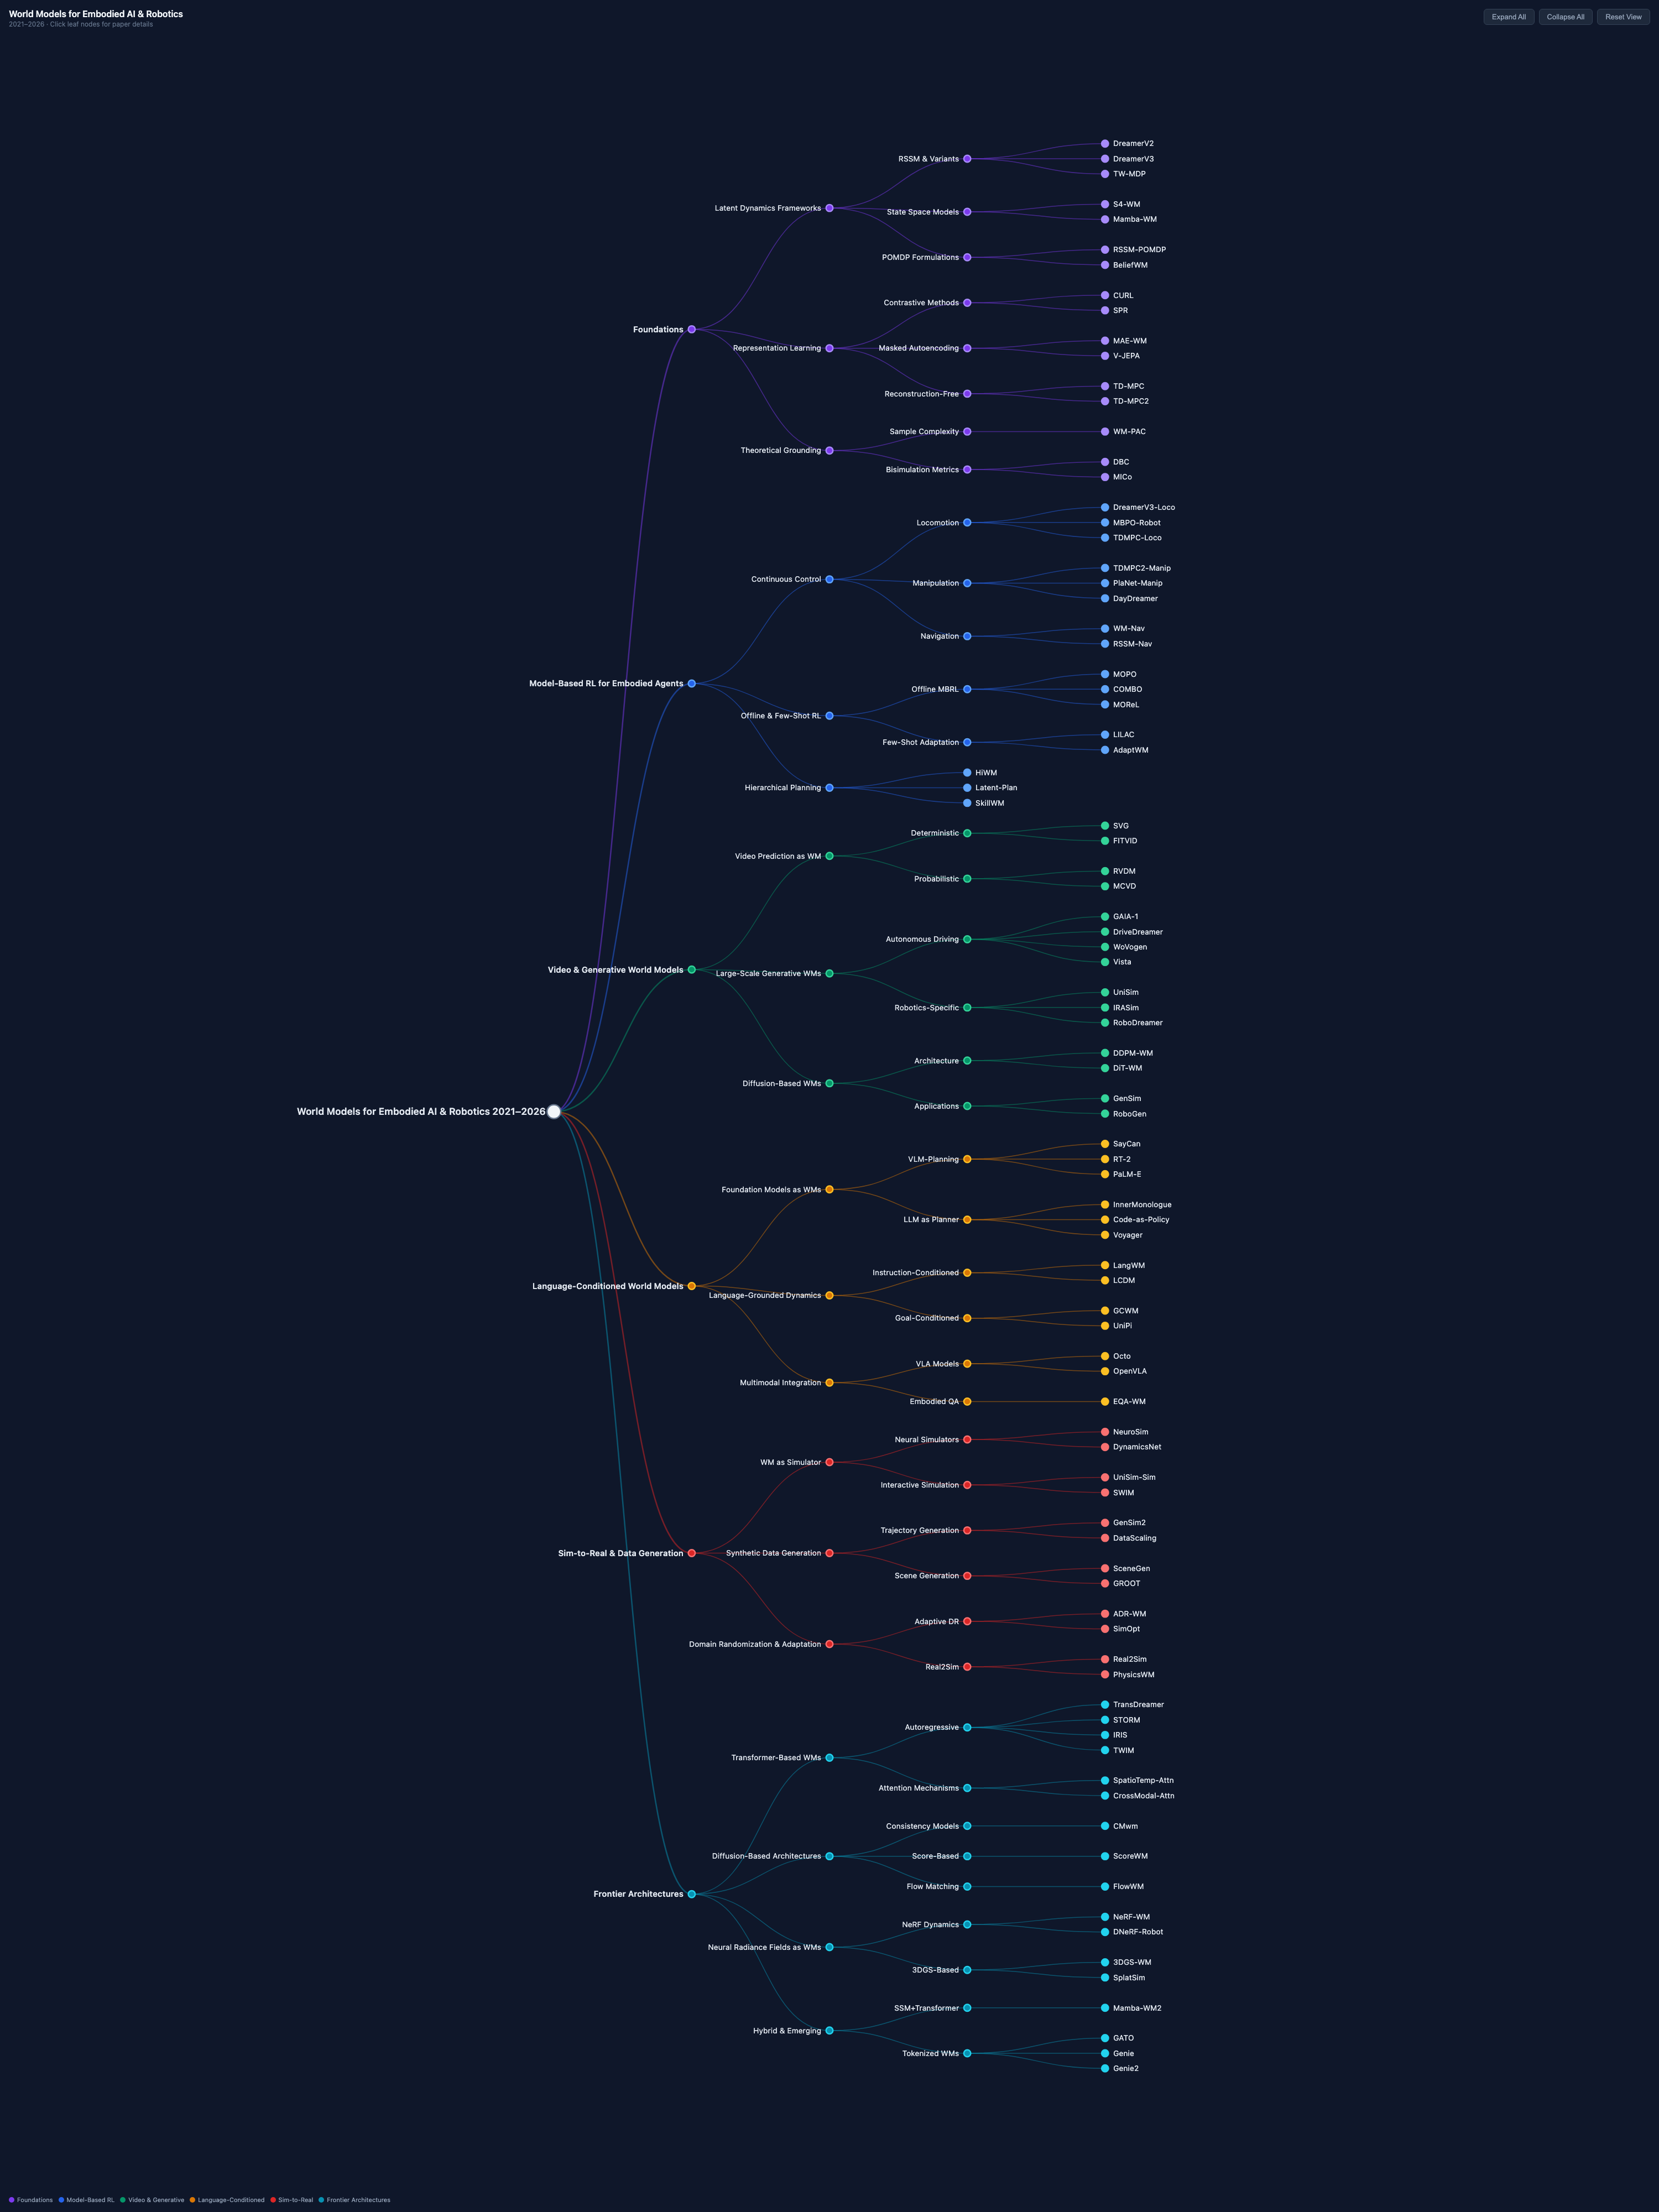
\includegraphics[width=0.95\textwidth]{case4/mindmap.png}
    \caption{Mind map generated autonomously by OMC's research team, covering six themes (Foundations, Model-Based RL, Video/Generative, Language-Conditioned, Sim-to-Real, Frontier Architectures) with approximately 70 nodes referencing 35+ papers from 2021--2026.}
    \label{fig:research-mindmap}
\end{figure}


\section{Research Survey: Generated Ideas}
\label{sec:research-ideas}

The three research ideas below were generated autonomously by OMC's research team, grounded in the failure modes (FM) identified during the survey.  The FM codes refer to entries in the team's failure mode taxonomy: FM-001 (compounding prediction error), FM-002 (physical implausibility), FM-003 (sim-to-real domain shift), and FM-008 (overconfident hallucination).

\subsection*{Idea 1: HiTeWM (Hierarchical Temporal World Models)}
\textbf{Problem}: Compounding prediction error (FM-001)---DreamerV3 degrades beyond 15 steps; RoboDreamer achieves only 15\% success on long-horizon tasks.  \textbf{Approach}: Two-level architecture with a fast model (50 Hz, RSSM-style, $\sim$50M params) for short-horizon dynamics and a slow model (2 Hz, Transformer-based) for macro-state transitions.  An uncertainty-gated re-grounding mechanism injects real observations when ensemble disagreement exceeds a learned threshold, converting pure imagination into closed-loop prediction.  \textbf{Expected improvement}: 30--50\% on 100+ step tasks vs.\ DreamerV3.

\subsection*{Idea 2: PhysWM (Physics-Grounded Latent World Models)}
\textbf{Problem}: Physical implausibility (FM-002)---video-based world models generate trajectories that violate conservation laws and contact constraints.  \textbf{Approach}: A Physics Constraint Module injects differentiable physics priors (rigid-body dynamics, energy conservation) into the latent transition function as soft penalties.  \textbf{Expected improvement}: 40--60\% in physical plausibility score; 20--35\% on contact-rich manipulation tasks.

\subsection*{Idea 3: MAWM (Meta-Adaptive World Models)}
\textbf{Problem}: Sim-to-real domain shift (FM-003) compounded by overconfident hallucination (FM-008).  \textbf{Approach}: Meta-learning across randomised sim domains produces an initialisation that adapts with $K{=}5$ real trajectories.  Conformal prediction provides calibrated uncertainty bounds, preventing the planner from acting on hallucinated predictions.  \textbf{Expected improvement}: $>$80\% task success with $K{=}5$ vs.\ $\sim$50--65\% baseline.